\section{Ergebnisse}

\subsection{Optimierung der Hyperparameter}

\subsubsection{Anzahl an Episoden}
\begin{itemize}
    \item Q-Learning\\
    Der in Abbildung \ref{fig:NumOfEpisods_Taxi} dargestellt Graph ziegt den Trainingsverlauf von Q-Learning bei dem Taxiproblem. Dort lässt sich erkennen das sich der Reward ab Episode 1300 kaum noch verändert, der Agent dementsprechend nicht mehr dazulernt. 
    Dieser Punkt wird als optimalen Wert für die maximale Anzahl an Episode angenommen.

    Um den optimalen Wert für das Cliff und Frozen Lake Problem zu ermitteln, wurden dieselben Schritte durchgeführt.
    Das Cliff Problem wird schneller von Agent erlernt, daher kann das Training schon nach etwa 1000 Episoden beendet werden.
    Der Trainingsverlauf des Frozen Lake Problem hat aufgrund der besonderen Rewardstruktur einen anderen Wertebereich (vgl. Abbildung \ref{fig:NumOfEpisods_Lake} ), ein Wert von etwa 600 benötigten Episoden lässt sich trotzdem problemlos ablesen.
    
    \begin{figure}[H]
      \centering
      \begin{subfigure}{.5\textwidth}
        \centering
        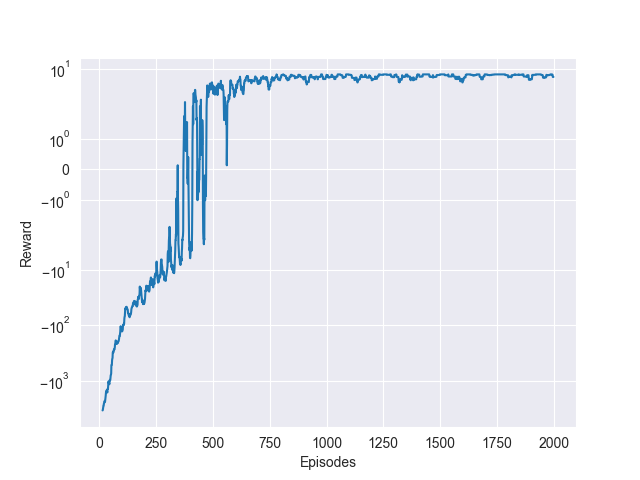
\includegraphics[width=1\linewidth]{Hyper_NumOfEpisods_Taxi}
        \caption{Trainingsverlauf Taxiproblem}
        \label{fig:NumOfEpisods_Taxi}
      \end{subfigure}%
      \begin{subfigure}{.5\textwidth}
        \centering
        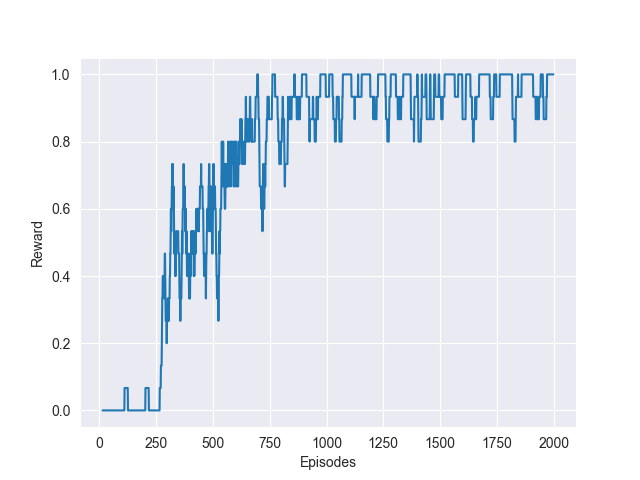
\includegraphics[width=1\linewidth]{Hyper_NumOfEpisods_Lake}
        \caption{Trainingsverlauf Frozen Lake}
        \label{fig:NumOfEpisods_Lake}
      \end{subfigure}
      \caption{Ermittlung der optimalen Anzahl an Episoden}
      \label{fig:NumOfEpisods_Taxi_Q-Learning}
  \end{figure}

    \item SARSA\\
    Das Verhalten von SARSA auf dem Taxiproblem ist sehr indentisch zu dem von Q-Learning, daher sind ist auch hier ein Wert von 1300 optimal.
    Bei dem Cliffproblem konvergiert der Reward ab 600 Epochen und beim FrozenLake Problem erzielt der Agent ab 2000 Epochen keinen Fortschritt mehr.
    In Abbildung \ref{fig:SARSA_NumOfEpisods} ist der Traingsverlauf von dem Cliffproblem (blau) und dem ForzenLake Problem (Orange) zu dargestellt.
    \begin{figure}[H]
      \centering
      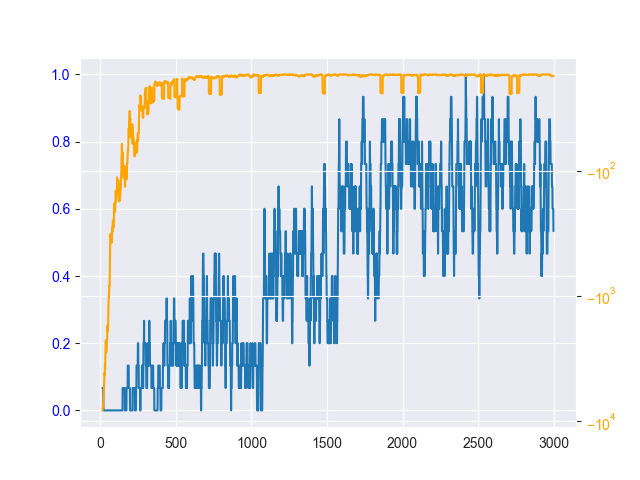
\includegraphics[scale=0.7]{Hyper_NumOfEpochs_Multi_SARSA}
      \caption{SARSA Traingsverlauf}
      \label{fig:SARSA_NumOfEpisods}
  \end{figure}
\end{itemize}

\subsubsection{Maximale Anzahl an Steps pro Episode}
\begin{itemize}
    \item Q-Learning\\
    Abbildung \ref{fig:MaxStepCount_1000vs500} stellt den Vergleich der Trainingsverläufe auf dem Taxiproblem zwischen den anfänglichen 1000 Steps zu 500 Steps dar.
    Diese deutliche Reduzierung der maximalen Steps hat zu folge, dass der Agent länger ein unstabiles Verhalten aufzeigt, somit ist diese Veränderung nicht sinnvoll.
    Abbildung \ref{fig:MaxStepCount_1000vs2000} zeigt den Effekt deiner Verdopplung des Wertes auf 2000. Zu erkennen ist, dass der Agent in der Mitte des Trainings schneller lernt, diesen Vorsprung verliert er gegen Ende des Trainings jedoch wieder.
    Bei genauerer Betrachtung lässt sich zu dem feststellen, dass der Verlauf gegen Ende etwas weniger schwankt, und somit der Agent minimal bessere Performance nach dem Training zeigen wird. 
    Eine weitere Erhöhung der maximalen Anzahl an Steps führte in den Versuchen allerdings nicht zu einer Verbesserung des Ergebnisses, verursachtet jedoch höhere Trainingszeiten.
    Zweittausend wurde somit als optimalen Wert für diesen Hyperparameter für das Taxi-Problem ermittelt. 

    \begin{figure}[H]
        \centering
        \begin{subfigure}{.5\textwidth}
          \centering
          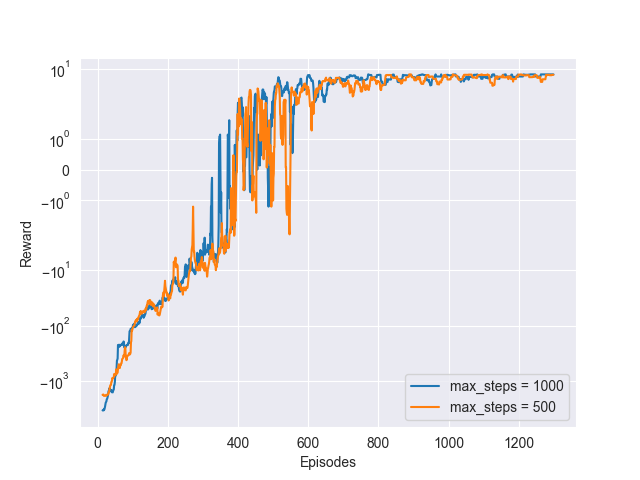
\includegraphics[width=1\linewidth]{Hyper_StepsPerEpisode_1000vs500}
          \caption{Vergleich 1000 vs 500}
          \label{fig:MaxStepCount_1000vs500}
        \end{subfigure}%
        \begin{subfigure}{.5\textwidth}
          \centering
          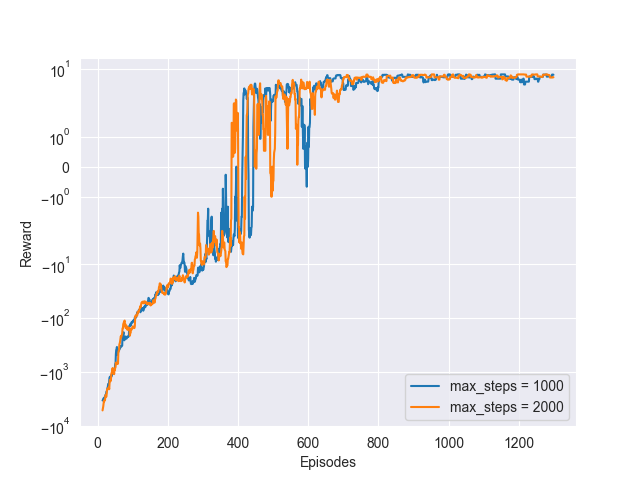
\includegraphics[width=1\linewidth]{Hyper_StepsPerEpisode_1000vs2000}
          \caption{Vergleich 1000 vs 2000}
          \label{fig:MaxStepCount_1000vs2000}
        \end{subfigure}
        \caption{Auswirkung der maximalen Anzahl an Episode}
        \label{fig:MaxStepCount}
    \end{figure}

    Für das Cliff Problem kann mit einem Wert von 750 schon das beste Ergebnis erzielt werden. 
    Dies hängt mit der durchschnittlich niedrigeren Anzahl an Steps, die zum Lösen des Problems benötigt werden, zusammen. 
    Bei der Untersuchung des Frozen Lake Problems konnte kein signifikanter Einfluss des Hyperparameters festgestellt werden, um Trainingszeit, die Trainingszeit gering zu halten wurde 500 als Wert festgelegt.
    \item SARSA\\
    Die Auswirkung der maximalen Steps auf SARSA bei dem Taxiproblem sind vergleichbar mit Q-Learning, verschiedene Versuche habe gezeigt, dass 2000 ein guter Wert für diesen Hyperparameter dargestellt.
Auf das Cliff Problem hat dieser Parameter kaum einen Einfluss, sodass der initiale Wert beibehalten werden kann.
Bei der Lösung der Frozen Lake Problems verbessert die Erhöhung der maximalen Steps das Ergebnis, als optimalen Wert wurde dabei erneut 2000 gewählt.
\end{itemize}
\subsubsection{Learning Rate}
\begin{itemize}
    \item Q-Learning\\
    Bei dem Vergleich verschiedener Learning Rates konnte festgestellt werden, dass Werte im Wertebereich zwischen 0,1 und 0,8 keinen Einfluss auf das Ergebnis des Trainings haben (vlg. Abbildung \ref{fig:learningRate_all}).
    Es kommt zwar zu kleinen Unterschieden in der Mitte des Trainings, diese sind aber eher auf die zufällig Exploration zurückzuführen.
    Eine zu kleine Learning Rate, wie Abbildung \ref{fig:learningRate_low} mit einem Wert von 0.01 veranschaulicht, führt jedoch zu einem längeren Trainingsverlauf.
    Für die weiteren Versuche wurde ein Wert von 0,4 festgelegt, da er sich in der Mitte des untersuchten Intervalls befindet.

    \begin{figure}[H]
        \centering
        \begin{subfigure}{.5\textwidth}
          \centering
          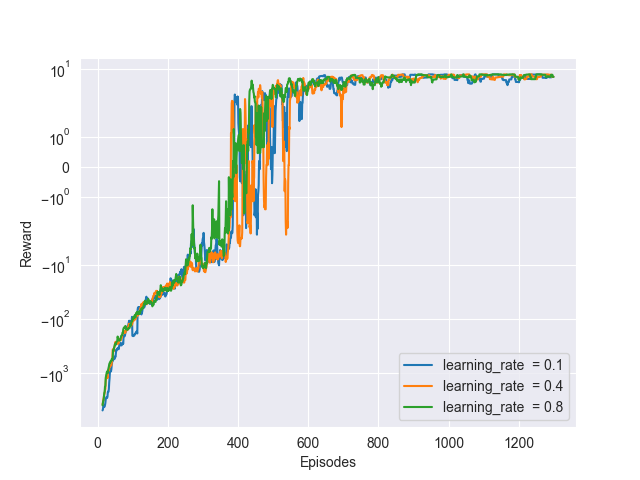
\includegraphics[width=1\linewidth]{Hyper_LearningRate_all}
          \caption{Einfluss Learning Rate}
          \label{fig:learningRate_all}
        \end{subfigure}%
        \begin{subfigure}{.5\textwidth}
          \centering
          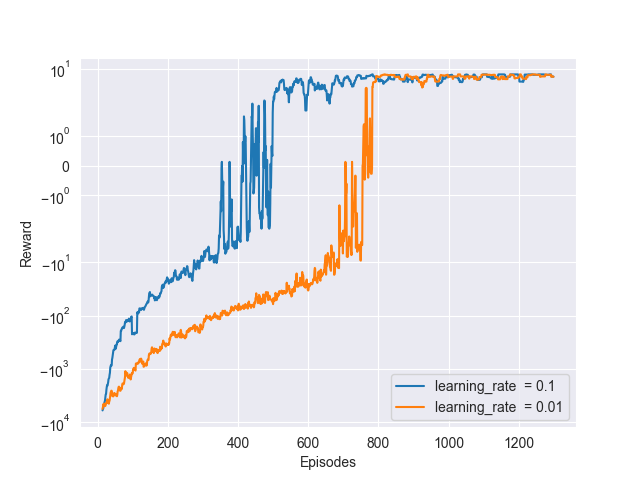
\includegraphics[width=1\linewidth]{Hyper_LearningRate_001}
          \caption{Wahl einer zu geringen Learning Rate}
          \label{fig:learningRate_low}
        \end{subfigure}
        \caption{Auswirkung der Learning Rate}
        \label{fig:learningRate_Q-Learning}
    \end{figure}
    \item SARSA\\
    Das Anheben der Learning Rate bei dem Taxiproblem führte bei SARSA sehr schnell zu einem unstabilen Verhalten, eine Reduktion verlangsamte das Training.
  	Somit führte keine Veränderung des Parameters zu einem bessern Ergebnis, und der initiale Wert wird beibehalten.
    Bei dem Cliff Problem für das Anheben erneut zu unstabilen Verhalten, die Reduzierung verbesserte jedoch das Ergebnis leicht, somit wurde ein Wert von 0,05 gewählt.
    Das Frozen Lake Problem konnte mit einer leicht erhöhten Learning Rate von SARSA besser gelöst werden, und es wurde final ein Wert von 0,3 festgesetzt.
\end{itemize}
\subsubsection{Discount Faktor}
\begin{itemize}
    \item Q-Learning\\
    Eine Reduzierung der Discount Rate auf 0,6 führte bei Q-Learning und dem Taxiproblem zu einem konstanteren Trainingsverlauf (vgl. Abbildung \ref{Hyper_DiscountRate_06}).
    Die Auswirkung einer weiteren Reduzierung des Parameters auf 0,2 ist Abbildung \ref{fig:DiscountRate02} zu entnehmen und führte zur leichten Verschlechterung des Ergebnisses.
    Da der Wert von 0,6 die besten Ergebnisse lieferte, wird dieser Wert für die folgenden Versuche verwendet.
    \begin{figure}[H]
        \centering
        \begin{subfigure}{.5\textwidth}
          \centering
          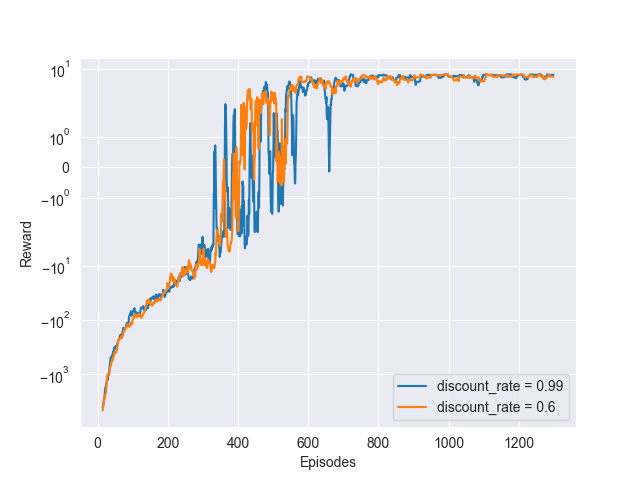
\includegraphics[width=1\linewidth]{Hyper_DiscountRate_06}
          \caption{Vergleich zwischen 0,99 vs 0,60}
          \label{fig:DiscountRate06}
        \end{subfigure}%
        \begin{subfigure}{.5\textwidth}
          \centering
          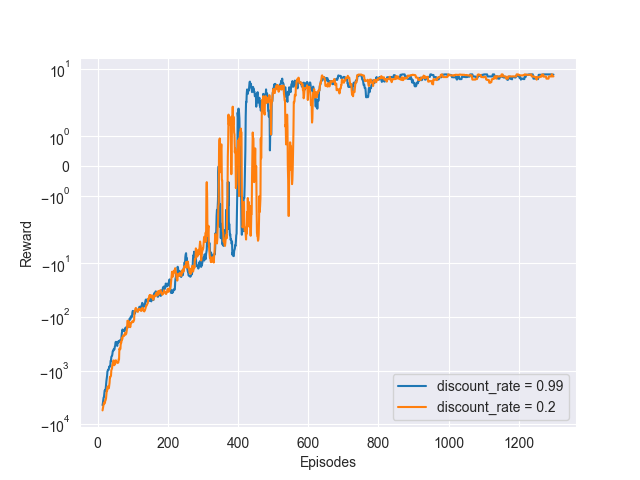
\includegraphics[width=1\linewidth]{Hyper_DiscountRate_02}
          \caption{Vergleich zwischen 0,99 vs 0,20}
          \label{fig:DiscountRate02}
        \end{subfigure}
        \caption{Auswirkung der Discount Rate}
        \label{fig:DiscountRate_Q-Learning}
    \end{figure}
    Bei dem Cliff Problem führt eine Absenkung des Wertes zu einer minimalen Verschlechterung der Ergebnisse, somit wird der Ausgangswert als Optimal angenommen. 
    Dieser hohe Initialwert verursachte bei dem Lake Problem häufiger einen Leistungseinbruch, der Agent war dann nicht mehr in der Lage, die Aufgabenstellung zu lösen.
    Durch eine Reduzierung des Wertes auf 0,2 konnte dieses Problem behoben werden.
    \item SARSA\\
    Eine Reduzierung des Hyperparameter führte beim Taxiproblem zu deutlich schlechteren Ergebnissen, da der initiale Wert bereits sehr nah am Maximum liegt, wurde dieser übernommen.
Ähnliches Verhalten zeigte sich auch bei der Untersuchung des Cliff Problems und von Frozen Lake, somit blieb auch dort der Parameter unverändert.
\end{itemize}
\subsubsection{Exploration Rate}

\begin{itemize}
  \item Q-Learning\\
  In Experimenten mit dem Taxiproblem hat sich gezeigt, dass eine Reduzierung der Exploration Decay Rate zu einem längeren Training führt, ohne dabei am Ende mehr Stabilität zu bringen (vgl. Abbildung \ref{fig:ExplorationDecayRate_low}).
  Das Erhöhen hingegen beschleunigt das Training minimal (vgl. Abbildung \ref{fig:ExplorationDecayRate_high}).
  Um ein schnelles Training zu erreichen und zeitlich sicherzustellen, dass der Agent alle möglichen Wege erkundet, wurde ein Wert von 0,01 für dieses Hyperparameter gewählt.
  Das Verhalten von Q-Learning auf dem Cliff Problem ist sehr identisch, daher ist auch dort 0,01 ein gut geeigneter Wert.
  Durch den hohen, auf Zufall basierender, Einfluss des Environments bei dem Frozen Lake Problems ist der Einfluss der Exploration Decay Rate nur in Extremfällen feststellbar.
  Daher wurde keine Anpassung des Standardwertes vorgenommen.
  \begin{figure}[H]
    \centering
    \begin{subfigure}{.5\textwidth}
      \centering
      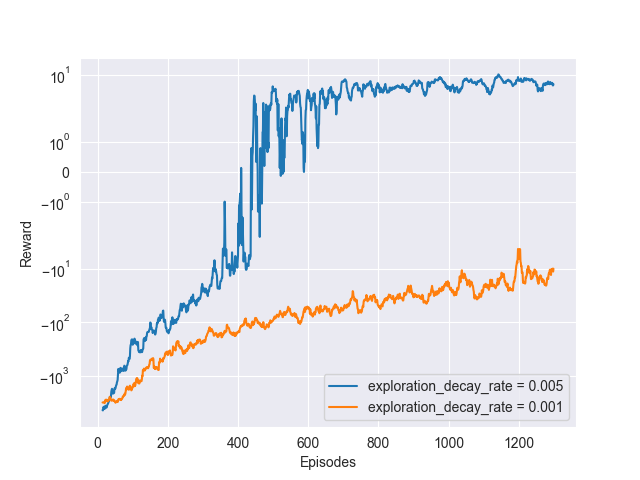
\includegraphics[width=1\linewidth]{Hyper_ExplorationDecayRate_001}
      \caption{Auswirkung niedriger Exploration Decay Rate}
      \label{fig:ExplorationDecayRate_low}
    \end{subfigure}%
    \begin{subfigure}{.5\textwidth}
      \centering
      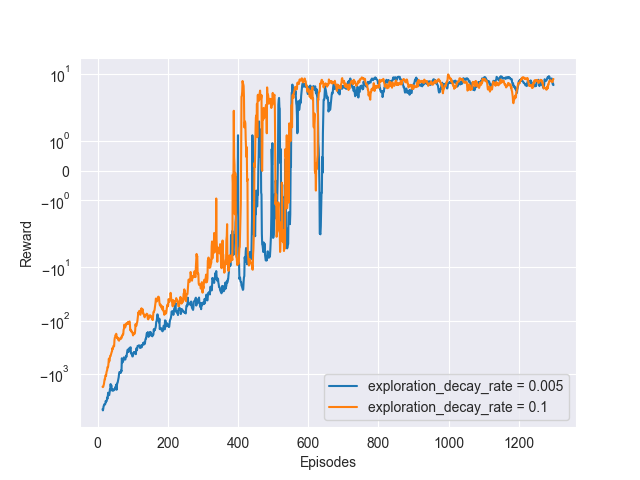
\includegraphics[width=1\linewidth]{Hyper_ExplorationDecayRate_01}
      \caption{Vergleich zwischen 0,99 vs 0,20}
      \label{fig:ExplorationDecayRate_high}
    \end{subfigure}
    \caption{Auswirkung der Exploration Decay Rate}
    \label{fig:ExplorationDecayRate_Q-Learning}
  \end{figure}
  \item SARSA\\
  Die Reduzierung der Exploration Decay Rate führt beim Taxiproblem und Cliff Problem, zu einem sehr Langsamen Training.
  Weitere Versuche Ergaben dass 0,1 auch für SARSA ein gutes Gleichgewicht zwischen Lerngeschwindigkeit und Exploration des Environments ist.
  Beim FrozenLake Problem überschattet der Zufallsfaktor des Environments jeglichen Einfluss dieses Parameters, somit bleibt der Wert unverändert.

\end{itemize}

\subsection{Vergleichen von Algorithmen}

Im folgenden werden die Ergebnisse beschrieben, welche bei dem Vergleichen der Algorithmen Q-Learning und SARSA entstanden sind.
Dabei wurde der Vergleich an den drei Reinforcement Learning Problemen Taxi, Cliff und Frozen Lake durchgeführt. Es wurden jeweils passende Paramater für das entsprechende Problem gewählt.
\subsubsection{Taxi}

In der Abbildung \ref{fig:taxi_train} sind die Ergebnisse für den Vergleich des Q-Learning und SARSA Algorithmus dargestellt. In der linken Abbildung \ref{fig:taxi_rew} sind die Rewards in dem zeitlichen Verlauf über die 3000 Trainingsepisoden abgebildet. Zu erkennen ist hier, dass beide Algorithmen nach ca. 1500 Episoden Richtung Optimum konvergieren. Der Q-Learning Algorithmus trainiert jedoch ein wenig schneller, was durch die anfänglich stärkere Steigung und höheren Peaks zu Beginn verdeutlicht wird.

Zusätzlich ist es auffällig, dass SARSA im späteren Verlauf auch größere Peaks nach unten hate und generell ein wenig schlechter performiert als der Q-Learning Algorithmus. Somit lässt sich insgesamt für die Belohnung feststellen, dass Q-Learning schneller zu einem besseren Ergebnis kommt als SARSA. 

In der zweiten Abbildung \ref{fig:taxi_step} sind die Anzahl der Steps abgebildet, welche der Agent jede Episode durchläuft, bis er entweder bei der maximalen Anzahl angekommen ist oder den Passagier erfolgreich zu seinem Zielort gebracht hat. Der Verlauf der beiden Kurven von Q-Learning und SARSA ist hier sehr ähnlich. Lediglich bei ca. 400 Episoden und 1300 lassen sich leicht höhere Peaks vom SARSA Algorithmus ablesen.
Dies spricht dafür, dass SARSA in diesen Phasen etwas langsamer gelernt hat als der Q-Learning Algorithmus.

Wichtig zu erwähnen ist zusätzlich, dass beide Algorithmen nach 3000 Episoden im Test perfekt opimiert sind. Im Test nutzen die trainierten Modelle keine Exploration Rate mehr, sondern gehen lediglich den Weg mit den höchsten Q-Values. Dies führt bei dem Taxi Problem bei beiden Algorithmen zu sehr ähnlichen Ergebnissen. Starten beide in dem gleichen State, laufen sie die fast die gleichen Wege um den Passagier abzuholen und zum Ziel zu bringen.

\begin{figure}[H]
    \centering
    \begin{subfigure}{.5\textwidth}
      \centering
      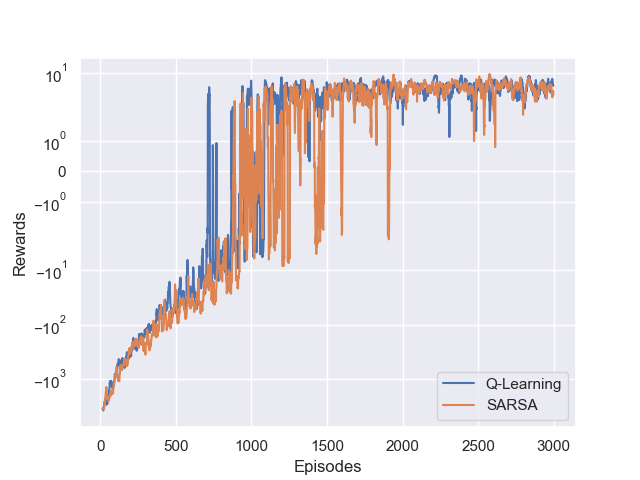
\includegraphics[width=1\linewidth]{taxi_q_vs_s_3000}
      \caption{Rewards}
      \label{fig:taxi_rew}
    \end{subfigure}%
    \begin{subfigure}{.5\textwidth}
      \centering
      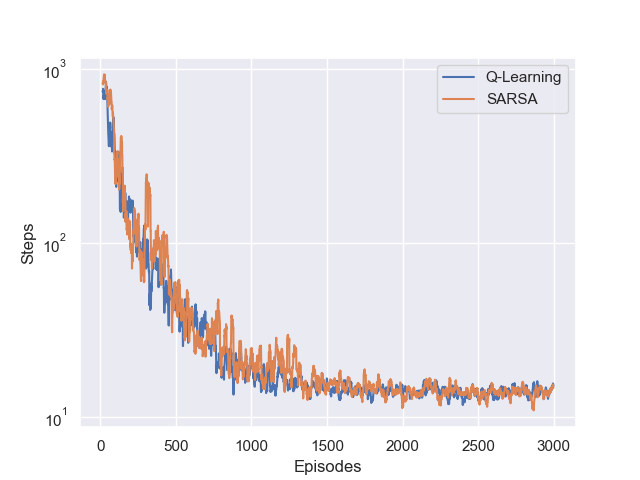
\includegraphics[width=1\linewidth]{taxi_q_vs_s_3000_steps}
      \caption{Steps}
      \label{fig:taxi_step}
    \end{subfigure}
    \caption{Taxi Problem über 3000 Episoden während dem Training}
    \label{fig:taxi_train}
\end{figure}

\subsubsection{Cliff}

Mit dem Cliff Problem lässt sich einer der besonderen Unterschiede zwischen Q-Learning und SARSA sehr gut zeigen. In Abbildung \ref{fig:cliff_train} sind wie in dem vorherigen Beispiel der Verlauf der Rewards (Abbildung \ref{fig:cliff_rew}) und die Anzahl an Steps (Abbildung \ref{fig:cliff_step}) über die Episoden im Training dargestellt.

Bei den Rewards ist zu erkennen dass SARSA zum Einen schneller lernt, dass heißt die Kurve geht zu Beginn schneller nach oben. Zum Anderen stagniert es auf einem höheren Reward zum Ende hin. Auch in der Abbildung \ref{fig:cliff_step} lässt sich ein Unterschied feststellen. Zu Beginn Verlaufen Sie zwar sehr ähnlich zum Ende hin ist es aber auffällig, dass SARSA bei eine höheren Anzahl an Steps stagniert, während der Verlauf bei Q-Learning deutlich niedriger, aber auch mit mehr Schwankungen vorliegt.




\begin{figure}[H]
    \centering
    \begin{subfigure}{.5\textwidth}
      \centering
      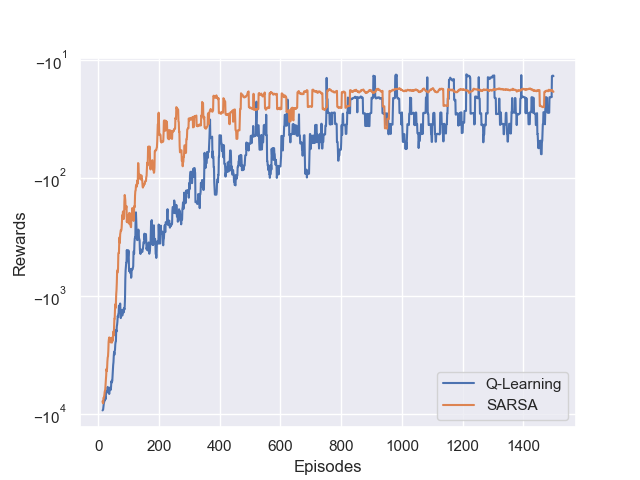
\includegraphics[width=1\linewidth]{cliff_q_vs_s_1500}
      \caption{Rewards}
      \label{fig:cliff_rew}
    \end{subfigure}%
    \begin{subfigure}{.5\textwidth}
      \centering
      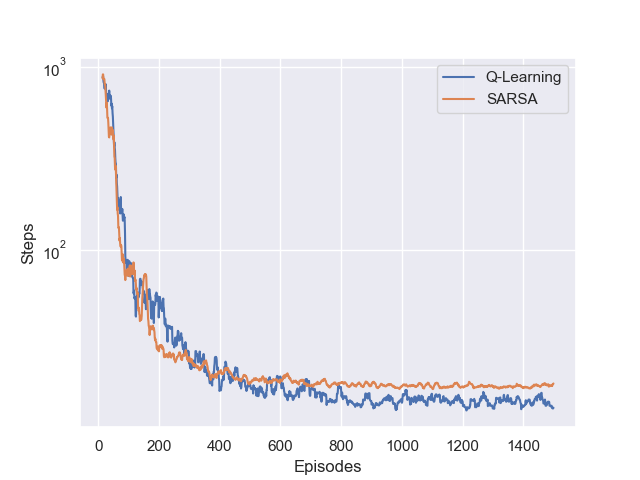
\includegraphics[width=1\linewidth]{cliff_q_vs_s_1500_steps}
      \caption{Steps}
      \label{fig:cliff_step}
    \end{subfigure}
    \caption{Cliff Problem über 1500 Episoden während dem Training}
    \label{fig:cliff_train}
\end{figure}

Dies liegt daran, dass SARSA ein on-policy Algorithmus ist. Dies bedeutet, dass es bei der Berechnung der Q-Value berücksichtigt, dass es eine Wahrscheinlichkeit gibt, zu der der Agent im nächsten Schritt explorieren statt exploiten wird.
Gerade bei dem Cliff Problem ist dies besonders spannend, da eine Exploration, welche in der Klippe endet, sehr fatal sein kann. In der Abbildung \ref{fig:cliff_path} sind die Wege dargestellt, welche die Algorithmen wählen. SARSA entscheidet sich aufgrund der on-policy Strategie für den ``safe path'' während Q-Learning für den ``optimal path'' geht. 
Beide Wege haben durchaus ihre Vor- und Nachteile und können je nach Anwendungsfall den subjektiv besseren Weg darstellen.
Aus den eben genannten Gründen nennt man Q-Learning auch einen greedy-Algorithmus, da er für den möglichst kürzten Weg geht, während SARSA etwas vorsichtiger, also weniger greedy, agiert.

\begin{figure}[H]
    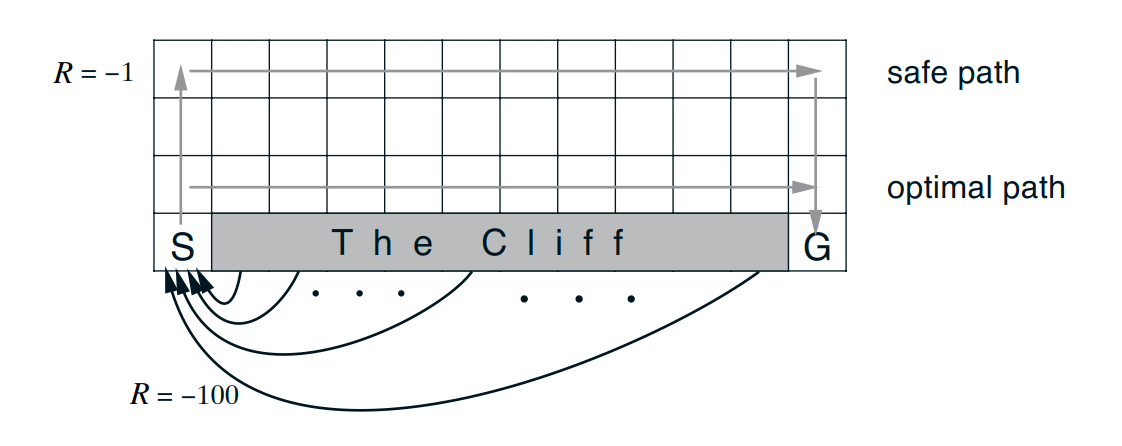
\includegraphics[scale=0.4]{cliff_path}
    \caption{Cliff Q-Learning vs SARSA Pfad}
    \label{fig:cliff_path}
\end{figure}

\subsubsection{Frozen Lake}

Das Frozen Lake Problem hat die Besonderheit, dass es nicht zu 100\% optimiert werden kann. Dies ist auch in den Abbildungen der Rewards (Abb. \ref{fig:frozen_rew}) und der Steps (Abb. \ref{fig:frozen_step}) zu erkennen. Beide Graphen verlaufen zwar jeweils ähnlich und stagnieren auf einem Niveau unter dem Optimum. Bezüglich der Unterschiede lässt sich hier kein sichtbarer Unterschied zwischen der Performance der Algorithmen aufzeigen. Bei den Rewards brauchen beide Algorithtmen ca. 500 Episoden um das Zielfeld regelmäßiger zu finden. Nach 2000 Episoden schaffen beide es teilweise zu 80\% während des Trainings. 
Anhand des Step Graphen ist zu erkennen, dass beide Algorithmen zu Beginn schnell in eines der Löcher fallen und somit die Episoden frühzeitig enden. Über die Zeit schaffen sie es aber länger auf dem Frozen Lake zu laufen. Optimalerweise würde die Anzahl der Steps gegen Ende wieder etwas sinken, dies ist aber in den ersten 2000 Episoden nicht der Fall.


\begin{figure}[H]
    \centering
    \begin{subfigure}{.5\textwidth}
      \centering
      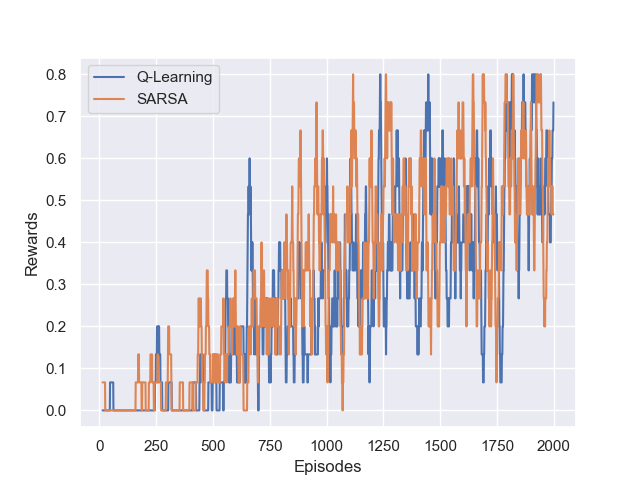
\includegraphics[width=1\linewidth]{frozen_lake_q_vs_s_2000}
      \caption{Rewards}
      \label{fig:frozen_rew}
    \end{subfigure}%
    \begin{subfigure}{.5\textwidth}
      \centering
      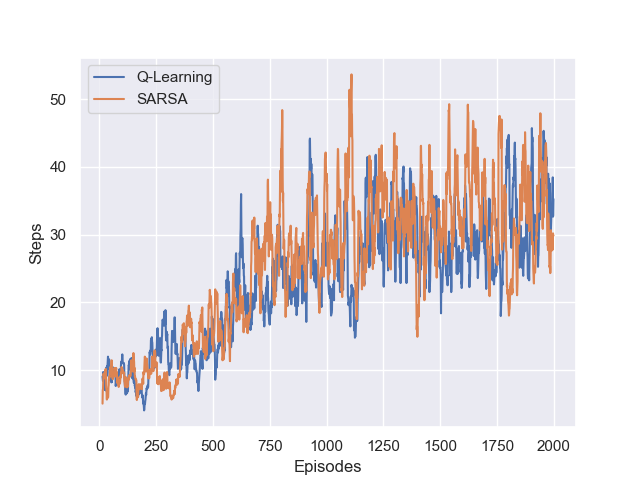
\includegraphics[width=1\linewidth]{frozen_lake_q_vs_s_2000_steps}
      \caption{Steps}
      \label{fig:frozen_step}
    \end{subfigure}
    \caption{Frozen Lake Problem über 2000 Episoden während dem Training}
    \label{fig:frozen_train}
\end{figure}

Dies kann daran liegen, dass das Environment durch den Zufallsparameter $is\_slippery = True$ für sehr zufällige Episoden sorgt. Dies ist auch daran zu erkennen, dass trotz des Rolling Windows, die Graphen sehr stark schwanken.

